On considère ci-dessous la représentation graphique d'une fonction $f$ définie sur $[-2~;~4]$. On a également tracé sa tangente au point $A$ d'abscisse $-1$.
	
	\medskip
	
	\begin{minipage}{0.46\linewidth}
		\begin{enumerate}
			\item Par lecture graphique, donner la valeur de :
			\begin{enumerate}
				\item $f(3)$
				
				\begin{color}{green!50!black}
				$f(3)\approx 5$
		 		\end{color}

				
				
				\item $f'(-1)$
				
				\begin{color}{green!50!black}
				$f'(-1)$ est donné par le coefficient directeur de la tangente à la courbe représentant $f$ au point d'abscisse $-1$.				
				
				$f'(-1)\approx 4$
		 		\end{color}
				
			\end{enumerate}
		\end{enumerate}
		
		
		
	\end{minipage}
	\hfill
	\begin{minipage}{0.5\linewidth}
		\centering
		\begin{tikzpicture}
			\begin{axis}[/pgf/number format/.cd, use comma,
				scaled ticks=false,
				x=8mm, y=8mm,
				xmin=-2.6, xmax=4.6, ymin=-0.6, ymax=9.8,
				axis lines=center,
				xtick={-3,-2,-1,0,1,2,3,4,5}, ytick={-1,0,1,2,3,4,5,6,7,8,9,10},
				tick label style={font=\scriptsize},
				minor tick num=1,
				grid=both,
				grid style={gray!70,dotted},
				clip=true]
				\addplot[teal,line width=1.5pt,samples=100,domain=-2:4]{-x^2+2*x+8};
				\fill[teal] (axis cs:-2,0) circle (1.5pt);
				\fill[teal] (axis cs: 4,0) circle (1.5pt);
				\addplot[red,line width=1.5pt,domain=-2.4:0.3]{4*x+9};
				\node[below left,font=\scriptsize] at (axis cs:0,0) {0};
				\node[above left,font=\footnotesize] at (axis cs:-1,5) {$A$};
				\node[font=\footnotesize,above left] at (axis cs:4.6,0) {$x$};
				\node[font=\footnotesize,below left] at (axis cs:0,9.8) {$y$};
				\filldraw (axis cs:-1,5) circle (1.5pt);
				\draw[orange,preaction={fill,opacity=0.5,fill=orange}] (axis cs:-1,5) -- (axis cs:0,9) -- (axis cs:0,5) node[midway, right] {\textbf{4}} -- cycle node[midway, below] {1} ;
				\draw[dashed, purple, opacity=0.5,line width=1.5pt] (axis cs:0,5) -- (axis cs:3,5) --  (axis cs:3,0) ;
				\node[rotate=45, purple,line width=1.5pt,draw,cross out,inner sep=0pt,minimum width=5pt,minimum height=5pt, opacity=0.7] at (axis cs:3,5) {};
				\node[purple,above right] at (axis cs:3,5) {$(3,\mathbf{5})$};
			\end{axis}
		\end{tikzpicture}
	\end{minipage}
	
	\begin{enumerate}[start=2]
			\item On admet que la fonction $f$ est définie sur $[-2~;~4]$ par \quad $f(x)=-x^{2}+2x+8$.
			\begin{enumerate}
				\item Calculer $f'(x)$ pour $x$ appartenant à $[-2~;~4]$.
				
				\begin{color}{green!50!black}
				$f'(x) = - (2\times x) + 2 \times 1 = -2x+2$
		 		\end{color}
				
			
				\item Étudier le signe de $f'(x)$ sur $[-2~;~4]$.
				
				\begin{color}{green!50!black}
				\[
				\begin{array}{ccc}
				-2x+2 = 0	 & \iff & 2x = 2 \\
						 & \iff & x = 1 \\
				\end{array}
				\]
				
				La fonction $f'$ est la restriction d'une fonction affine sur $[-2~;~4]$. Le taux d'accroissement est négatif donc elle est décroissante. Elle admet pour racine le nombre $1$. Ainsi $f'(x)$ est positif si $x$ est inférieur à $1$ et négatif si $x$ est supérieur à $1$.
				
				
		 		\end{color}
				
				
			\end{enumerate}
			\item Donner les variations de $f$ sur $[-2~;~4]$.
			
			\begin{color}{green!50!black}
			$f(-2) = -(-2)^2 +2\times(-2) + 8 = -4 - 4 + 8 =0$
						
			$f(4) = -4^2 +2\times 4 + 8 = -16 + 8 + 8 =0$
			
			$f(1) = -1^2 +2\times 1 + 8 = -1 + 2 + 8 = 9$
			
			\begin{tikzpicture}
				\tkzTabInit[lgt=3, espcl=4]{$x$ / 1, {signe de $f'(x)$} / 1.5, {variations de $f(x)$} / 3.5}{$\np{-2}$, $1$ , $4$}
				\tkzTabLine{,+,z,-,}
				\tkzTabVar{-/$0$ , +/$9$ , -/$0$ }
			\end{tikzpicture}
			\end{color}
				
			
		\end{enumerate}
	
	
	\medskip
